\documentclass[11pt,a4paper]{article}

\usepackage[utf8]{inputenc}
\usepackage[T1]{fontenc}
\usepackage{geometry}
\usepackage{graphicx}
\usepackage{booktabs}
\usepackage{hyperref}
\usepackage{caption}
\usepackage{float}

\geometry{margin=2.5cm}

\hypersetup{
    colorlinks=true,
    linkcolor=blue,
    urlcolor=blue,
    citecolor=blue
}

\title{\textbf{CLARISSA: A Conversational Agent Architecture for Democratizing Reservoir Simulation}}
\author{Wolfram Laube\\Independent Researcher, Austria}
\date{SPE Europe Energy Conference 2026\\Technical Category: Digitalization / Reservoir Simulation}

\begin{document}

\maketitle

\begin{abstract}
Reservoir simulation remains underutilized across the full spectrum of reservoir engineering---field development planning, production surveillance, forecasting, reserves booking, and exploration risking---despite decades of software advancement. The barrier is not computational; modern solvers are fast and robust. The barrier is accessibility.

This paper introduces \textsc{CLARISSA} (Conversational Language Agent for Reservoir Integrated Simulation System Analysis), a phased AI agent architecture that replaces the GUI paradigm with physics-aware conversational interaction. Rather than requiring users to navigate software, CLARISSA enables reservoir engineers to build and iterate on simulation models through natural language dialogue.

Recent work has demonstrated generative AI assistants that help engineers query existing models and retrieve simulator documentation (SPE-221987). CLARISSA addresses a different problem: generating complete, validated input decks from natural language specifications while maintaining simulator-in-the-loop feedback for physics-grounded reasoning. The architecture combines large language models for planning and human interaction, reinforcement learning for optimizing action sequences based on numerical outcomes such as convergence behavior, and neuro-symbolic components enforcing engineering constraints and safety boundaries.

CLARISSA integrates OPM Flow as primary execution backend, enabling a web-based service model accessible to operators without commercial simulation licenses. To enable systematic evaluation, we introduce \textsc{RIGOR} (Reservoir Input Generation Output Review), a benchmark framework assessing deck generation across four dimensions: syntactic validity, semantic correctness, physical plausibility, and conversational efficiency.

\textit{The binding constraint on simulation adoption has never been solver performance. It is human cognitive load and workflow friction. CLARISSA addresses that constraint directly.}
\end{abstract}

\textbf{Keywords:} Reservoir Simulation, Generative AI, Large Language Models, Natural Language Processing, OPM Flow, Conversational Agents, Deck Generation

\section{Architecture Overview}

The CLARISSA system architecture comprises four primary layers: User Interface, Core Processing, Simulation, and Knowledge Management. Figure~\ref{fig:architecture} illustrates the component relationships.

\begin{figure}[H]
    \centering
    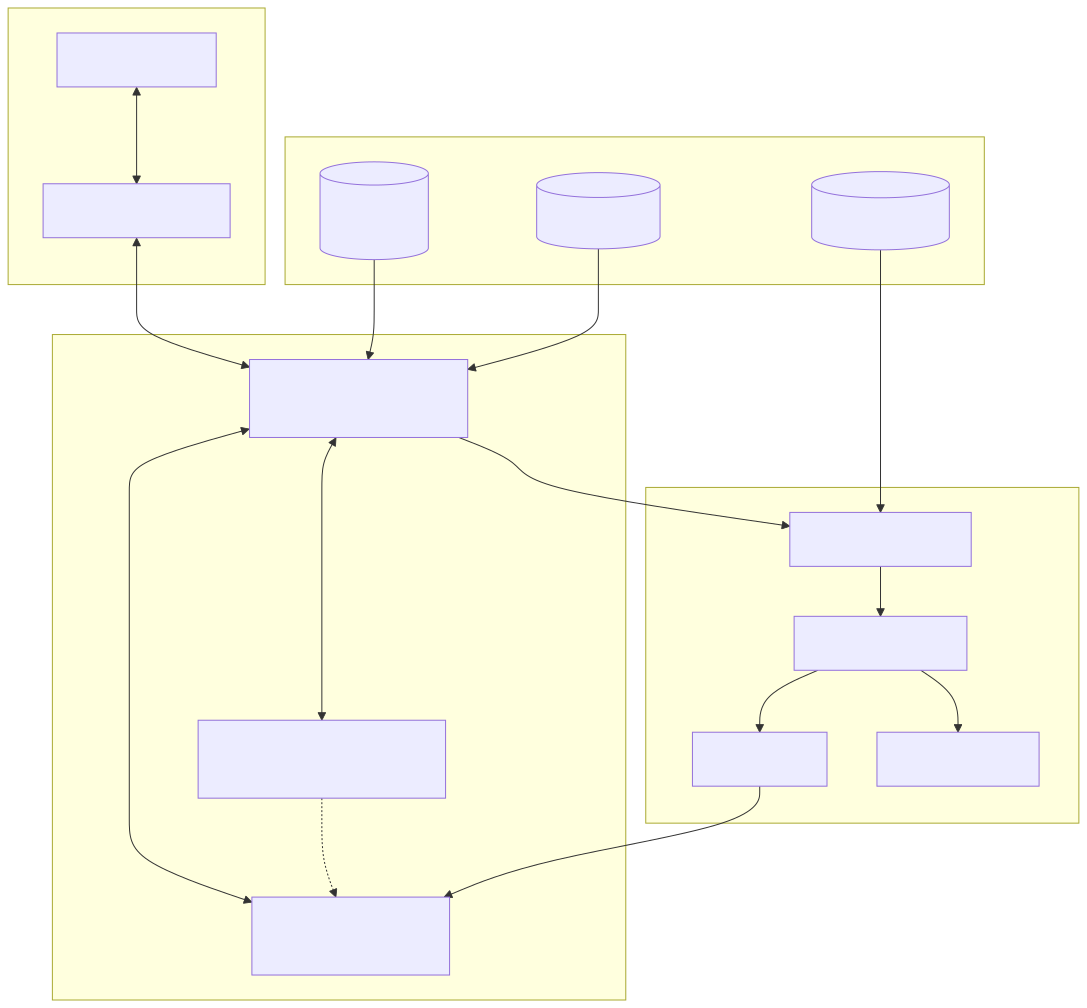
\includegraphics[width=0.9\textwidth]{diagrams/architecture.pdf}
    \caption{CLARISSA System Architecture showing the interaction between User Interface, Core (LLM, RL Agent, Neuro-Symbolic Constraints), Simulation (Validator, Generator, OPM Flow), and Knowledge layers.}
    \label{fig:architecture}
\end{figure}

\section{Development Phases}

CLARISSA evolves through three phases: syntactic assistance for deck generation and debugging, physics-informed support incorporating simulation feedback loops, and ultimately field-specialized agents embedded in operational teams. Figure~\ref{fig:phases} shows this progression.

\begin{figure}[H]
    \centering
    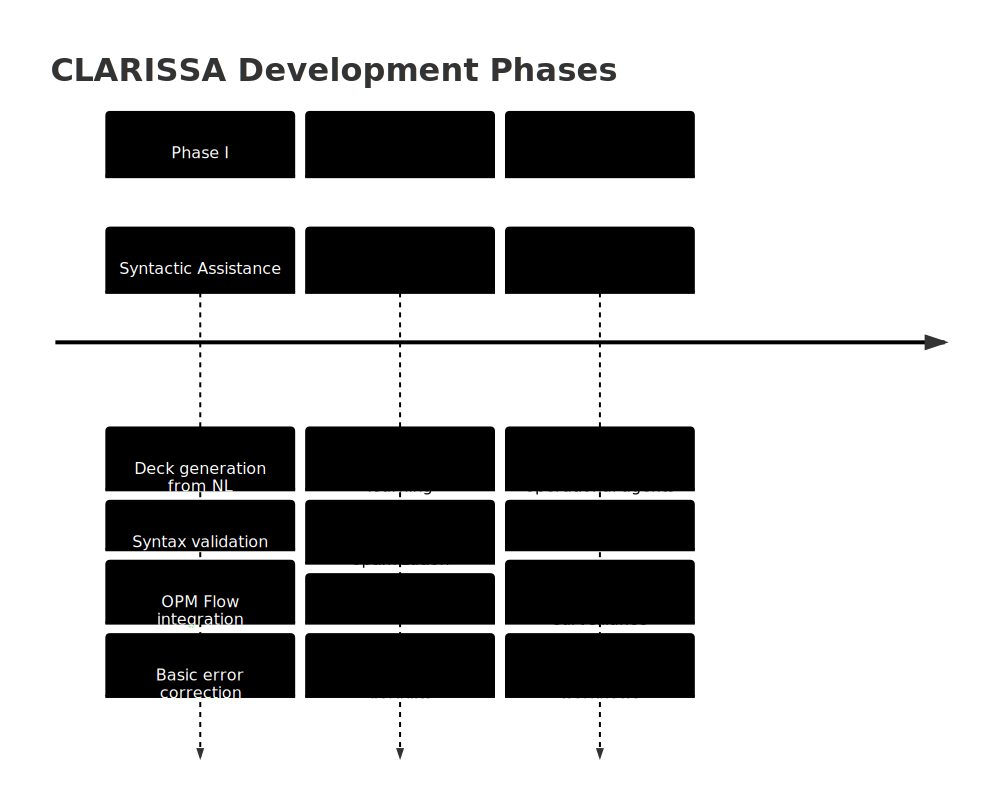
\includegraphics[width=0.85\textwidth]{diagrams/phases.pdf}
    \caption{CLARISSA Development Phases: Phase I (Syntactic Assistance), Phase II (Physics-Informed), and Phase III (Field-Specialized).}
    \label{fig:phases}
\end{figure}

\section{Comparison with Prior Work}

Figure~\ref{fig:comparison} and Table~\ref{tab:comparison} illustrate the key differences between CLARISSA and the Envoy system described in SPE-221987.

\begin{figure}[H]
    \centering
    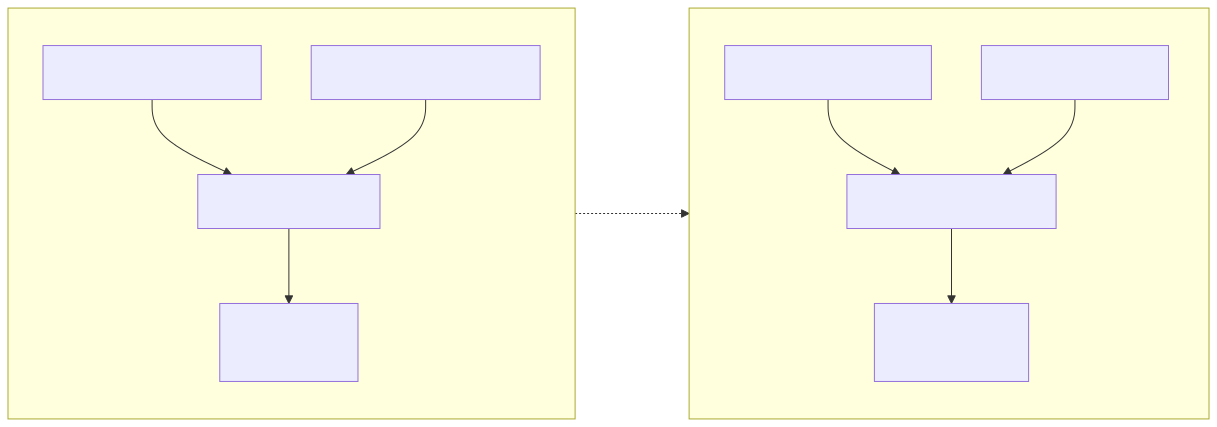
\includegraphics[width=0.8\textwidth]{diagrams/comparison.pdf}
    \caption{Evolution from Envoy (SPE-221987) to CLARISSA: Query-based vs. Generation-based approaches.}
    \label{fig:comparison}
\end{figure}

\begin{table}[H]
\centering
\caption{Feature Comparison: Envoy vs. CLARISSA}
\label{tab:comparison}
\begin{tabular}{lll}
\toprule
\textbf{Aspect} & \textbf{Envoy (SPE-221987)} & \textbf{CLARISSA} \\
\midrule
Primary Function & Query existing models & Generate complete decks \\
Interaction Mode & Q\&A on loaded model & Elicitation dialogue \\
Simulator & ECHELON (proprietary) & OPM Flow (open source) \\
Architecture & RAG + Callback Agents & RL + Neuro-symbolic + Loop \\
Learning & Static knowledge bases & Adaptive via sim feedback \\
Availability & Commercial license & Web-based, license-free \\
Validation & Post-hoc analysis & Pre-execution physics check \\
\bottomrule
\end{tabular}
\end{table}

\section{RIGOR Benchmark Framework}

To enable systematic evaluation, we introduce RIGOR (Reservoir Input Generation Output Review), illustrated in Figure~\ref{fig:rigor}.

\begin{figure}[H]
    \centering
    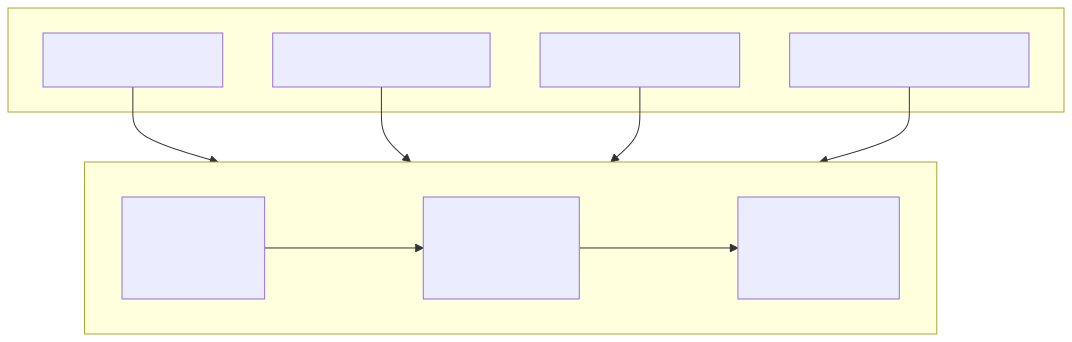
\includegraphics[width=0.75\textwidth]{diagrams/rigor.pdf}
    \caption{RIGOR Benchmark Framework: Four evaluation dimensions applied across three complexity tiers.}
    \label{fig:rigor}
\end{figure}

\section{Conversation Flow}

Figure~\ref{fig:conversation} demonstrates a typical interaction sequence between an engineer and CLARISSA.

\begin{figure}[H]
    \centering
    \includegraphics[width=0.95\textwidth]{diagrams/conversation.pdf}
    \caption{Example conversation flow showing iterative model specification, validation, and simulation execution.}
    \label{fig:conversation}
\end{figure}

\section{Technical Stack}

Figure~\ref{fig:techstack} shows the high-level technology components.

\begin{figure}[H]
    \centering
    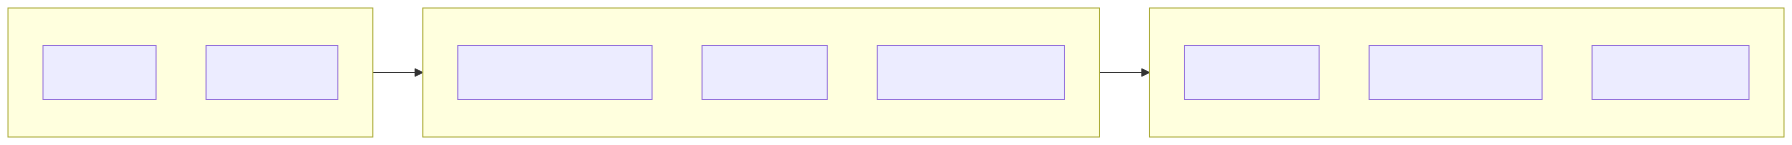
\includegraphics[width=0.7\textwidth]{diagrams/techstack.pdf}
    \caption{CLARISSA Technical Stack: Frontend, Core, and Simulation components.}
    \label{fig:techstack}
\end{figure}

\section{Conclusions}

CLARISSA represents a fundamental shift in how reservoir engineers can interact with simulation tools. By replacing the GUI paradigm with physics-aware conversational interaction, we address the accessibility barrier that has limited simulation adoption across the industry.

\begin{thebibliography}{9}
\bibitem{spe221987}
K. Wiegand, M. Bedewi, K. Mukundakrishnan, D. Tishechkin, V. Ananthan, and D. Kahn,
``Using Generative AI to Build a Reservoir Simulation Assistant,''
SPE-221987-MS, ADIPEC, Abu Dhabi, 2024.
\end{thebibliography}

\end{document}
